\documentclass[11pt,a4paper]{article}

\usepackage[utf8]{inputenc}
\usepackage[T1]{fontenc}
\usepackage{lmodern}
\usepackage{geometry}
\usepackage{xcolor}
\usepackage{enumitem}
\usepackage{listings}
\usepackage{booktabs}
\usepackage{longtable}
\usepackage{array}
\usepackage{graphicx}
\usepackage{microtype}
\geometry{margin=2.5cm}

\definecolor{codegray}{RGB}{245,245,245}
\definecolor{darkblue}{RGB}{20,60,120}

\usepackage[
  colorlinks=true,
  linkcolor=darkblue,
  urlcolor=darkblue,
  citecolor=darkblue,
  breaklinks=true
]{hyperref}

\lstdefinestyle{codestyle}{
  backgroundcolor=\color{codegray},
  basicstyle=\ttfamily\small,
  breaklines=true,
  frame=single,
  columns=fullflexible,
  keepspaces=true,
  showstringspaces=false,
  upquote=true
}

\newcommand{\code}[1]{\texttt{#1}}
\setlist{leftmargin=*}
\setlength{\LTpre}{0.5em}
\setlength{\LTpost}{0.5em}
\setlength{\emergencystretch}{3em}

\title{Demo Provenance-Aware Question Answering Gateway}
\author{}
\date{}

\begin{document}
\sloppy
\maketitle
\tableofcontents
\newpage

\section*{Abstract}


\section{Motivation and Objectives}

Large language models can translate questions, synthesize answers, and manipulate
structured representations, but a fluent answer alone does not show which source
records support it. For question answering task, a system
should output both the answer and the evidence used to derive it.

This demo has the following objectives:

\begin{itemize}
  \item answer questions over tabular datasets through several alternative pipelines;
  \item preserve stable row identifiers from source data through retrieval and generation;
  \item compute or explain provenance using the records that contributed to an answer;
  \item expose plans, retrieved context, prompts, model output, validation results,
        generated CSV files, and service responses for inspection; and
  \item provide a common OpenAI-compatible interface for comparing base,
        fine-tuned, planner-based, and internal-knowledge configurations.
\end{itemize}

\section{Related Work}

\subsection{Retrieval-Augmented Generation}

Retrieval over tabular data requires different design choices from standard document retrieval. A common approach in RAG systems is to linearize tables into text and retrieve them as ordinary chunks. However, recent work has shown that this strategy may lose important tabular structure and provide only a partial view of the data, especially for questions requiring joins, filtering or aggregation. TableRAG ~\cite{yu2025tableragretrievalaugmentedgeneration} addresses this limitation by combining text retrieval with SQL-based execution over tabular components for heterogeneous document reasoning, showing the importance of preserving the distinction between textual and structured evidence. During an offline phase, the system extracts table contents, builds textual chunks for retrieval, stores table schemas, and also ingests the tables into a relational database. During online inference, it decomposes the user question, retrieves relevant chunks, maps retrieved table fragments back to their corresponding schemas, generates SQL when tabular reasoning is required, executes the SQL query over the relational database, and combines the execution result with retrieved textual evidence to generate the answer.

Our retrieval component follows a related motivation, but adapts it to relational CSV data. Instead of indexing arbitrary table chunks, we create one document for each table row. Each document contains a textual representation of the row, including the table name, primary-key values, column-value pairs, and selected foreign-key links to related rows. This row-level representation is designed to preserve enough relational structure for retrieval while remaining compatible with dense vector search. In addition, the document metadata stores the original table, row identifier, primary key, full row values, provenance row number when available, and linked-row information. The resulting documents are embedded with BGE-M3 and indexed with FAISS, enabling the system to retrieve candidate records that can later be used by the LLM.

Our retrieval design is also influenced by schema-aware approaches such as RAT-SQL~\cite{ratsql}. RAT-SQL addresses text-to-SQL parsing by making the structure of the database schema explicit: tables and columns are represented as graph nodes, while relations such as primary keys, foreign keys, and column-table membership are encoded as graph edges. This allows the model to reason not only over the textual form of the schema, but also over the relational connections that determine how tables and columns should be interpreted.

Although our system does not adopt RAT-SQL's neural parser, it follows a similar principle at the retrieval level. Each indexed document is not a plain textual chunk, but a structured representation of a relational row. In this way, relational information that would be hidden or lost in a naive text representation is made explicit before embedding and retrieval.


\subsection{Data Provenance}

Data provenance, by explaining how the result of an operation is derived from its inputs, has proven to be a crucial concept across a wide variety of applications. As highlighted by \cite{bookProvenance}, provenance enables fundamental functionalities such as debugging queries and transformations, assessing the trustworthiness of data, interpreting complex data processing pipelines, and performing incremental maintenance of query results. It also supports explaining unexpected query outcomes and reasoning about hypothetical changes to inputs and outputs.

These are the core provenance models:
\textbf{Lineage} \cite{whyAndWhereBuneman}, based on data dependencies that track data dependencies separately for each input relation of a query.  Lineage focuses on identifying the specific input tuples that contribute to each output tuple. It provides an efficient way to trace data origin. The lineage is computed by breaking down the query into smaller parts, then computing which tuples in subqueries contributed to each intermediate result, and finally combining all their lineages to get the final answer.
\textbf{Why provenance} \cite{whyAndWhereBuneman}, which captures sets of input tuples (witnesses) that are sufficient to produce a particular output tuple. It reflects the minimal explanations of why an answer exists. 
\textbf{How provenance} \cite{whyHowWhereprovenance}, which goes further by expressing the precise combination and multiplicity of input tuples used to compute each output.
\textbf{Where provenance} \cite{whyAndWhereBuneman}, which focuses on the origin of individual data values. While why-provenance captures the relationship between source and output tuples, where provenance traces the exact source locations (specific rows in the input relations) from which output values are copied. This notion highlights the link between input and output attributes, but, unlike why provenance, it is not invariant under query equivalence.
Moreover, the article covers key algorithms for provenance tracking, the computational complexity of various provenance models, and the integration of provenance computation into query engines and data management systems.

One of the key techniques discussed in the article for tracking data provenance is the use of \textbf{semirings}, an algebraic framework that provides a unified way to compute and represent provenance information during query processing. A fundamental contribution in this field was achieved through the provenance \textbf{semiring framework} \cite{provenanceSemirings}, which models various forms of provenance, including why-provenance. In this framework, relations are annotated with elements of semirings and relational algebra operators are mapped to semiring operations.
Using the semiring framework, each tuple in the database is bound with a provenance annotation. As a query is executed, these annotations are propagated and combined according to the query's structure. What makes the semiring model powerful is that it defines two operations, addition and multiplication, to determine how provenance annotations should be handled at each step of the query.
Addition is used when a query operation (like a union) can produce the same output tuple in multiple ways. In this case, the provenance of the output is the combination of the alternative sources.
Multiplication is used when the result depends on the combination of multiple input tuples (as in a join). Here, the provenance of the result reflects the joint contribution of those inputs.

Our project is based on the notion of \textit{why-provenance}.
Why-provenance is a fundamental provenance model originally introduced by Buneman et al. (2001) \cite{whyAndWhereBuneman} to formalize the explanation of query results based on the principles of sufficiency and minimality. In this framework, the provenance of a query result is characterized by identifying subsets of the input database, called \textit{witnesses}, each of which alone suffices to produce that result.
\textbf{Witness sets} are derived from the semiring expression by enumerating the minimal input tuple combinations that are sufficient to produce the output tuple.
Each multiplicative term in the provenance polynomial corresponds to one witness set.
Formally, the \textit{set of witnesses} for a tuple $t$ in the output of a query $Q$ over a database $D$ is defined as the collection of all subsets $D' \subseteq D$ such that $t \in Q(D')$. Since this set can contain redundant witnesses that include unnecessary tuples, the notion of \textit{minimal witnesses} is introduced. Minimal witnesses are those subsets that are minimal under set inclusion, meaning they do not contain any smaller witness that also produces $t$. This minimality ensures the provenance explanations focus on essential and non-redundant parts of the input data.
We use this concept to enhance the interpretability of outputs produced by a Retrieval-Augmented Generation (RAG) pipeline. We use the notion of \textit{witness sets}, which act as textual justifications for each item of an answer, effectively mapping the output back to its supporting retrieved content. 
\subsection{Databases and LLMs}
Recent work has investigated how database query-processing ideas can be adapted to interactions with Large Language Models. Satriani et al. introduce Galois ~\cite{EURECOM+8182}, a system that executes SQL queries over LLMs by treating the model as a data source and by defining LLM-aware logical and physical operators. In particular, Galois introduces LLMScan and Filter-LLMScan operators, which retrieve tuples from the model either without or with pushed-down selection conditions. Their work shows that complex data-oriented queries can benefit from being decomposed into operator-level plans, and that deciding whether conditions should be pushed into the LLM call involves a trade-off between cost and result quality.

Our demo system takes inspiration from this operator-oriented view, but adapts it to a different setting. In our planner-based pipelines, we introduce analogous LeafScan and FilterLeafScan steps. These steps are applied to the leaves of a generated tree plan and are used to query the LLM on smaller tasks, optionally with filter conditions pushed into the leaf. Unlike Galois, however, our system does not treat the LLM as the primary storage layer. The data source remains an explicit collection of relational tables, and the LLM is used as part of a pipeline involving retrieval, planning, structured generation, deterministic execution, and provenance explanation.

This distinction is central to our use of the idea. While Galois studies how SQL execution can be optimized when the LLM itself is queried as a data source, our system studies how LLM calls can be organized around a planner when answering questions over existing tabular data. 

\section{System Architecture}

The deployed system contains the following services.

\begin{longtable}{>{\raggedright\arraybackslash}p{0.25\textwidth} >{\raggedright\arraybackslash}p{0.67\textwidth}}
\toprule
\textbf{Component} & \textbf{Responsibility} \\
\midrule
\endhead
FastAPI gateway & API routing, dataset loading, retrieval, planning, prompting,
validation, logging, UI hosting, and orchestration. \\
Ollama & Local serving of the base and fine-tuned Llama models. \\
OpenAI-compatible LLM endpoint & Optional provider for planner leaf calls, selected
through configuration. \\
FAISS & Dense row-level indexes, one index per configured dataset. \\
AP Explanation service & Loads generated CSV relations, executes the requested
query, and returns answer and provenance information. \\
PostgreSQL with ProvSQL & Relational execution and provenance support for the
explanation service. \\
Redis & Task broker and result backend used by the explanation service. \\
Shared bucket & File exchange area for generated per-table CSV files. \\
\bottomrule
\end{longtable}

The gateway and explanation service share \code{./bucket} through different
container mount points. A process-wide lock serializes explanation pipelines
because each run cleans and rewrites this shared directory.

\begin{figure}[htbp]
  \centering
  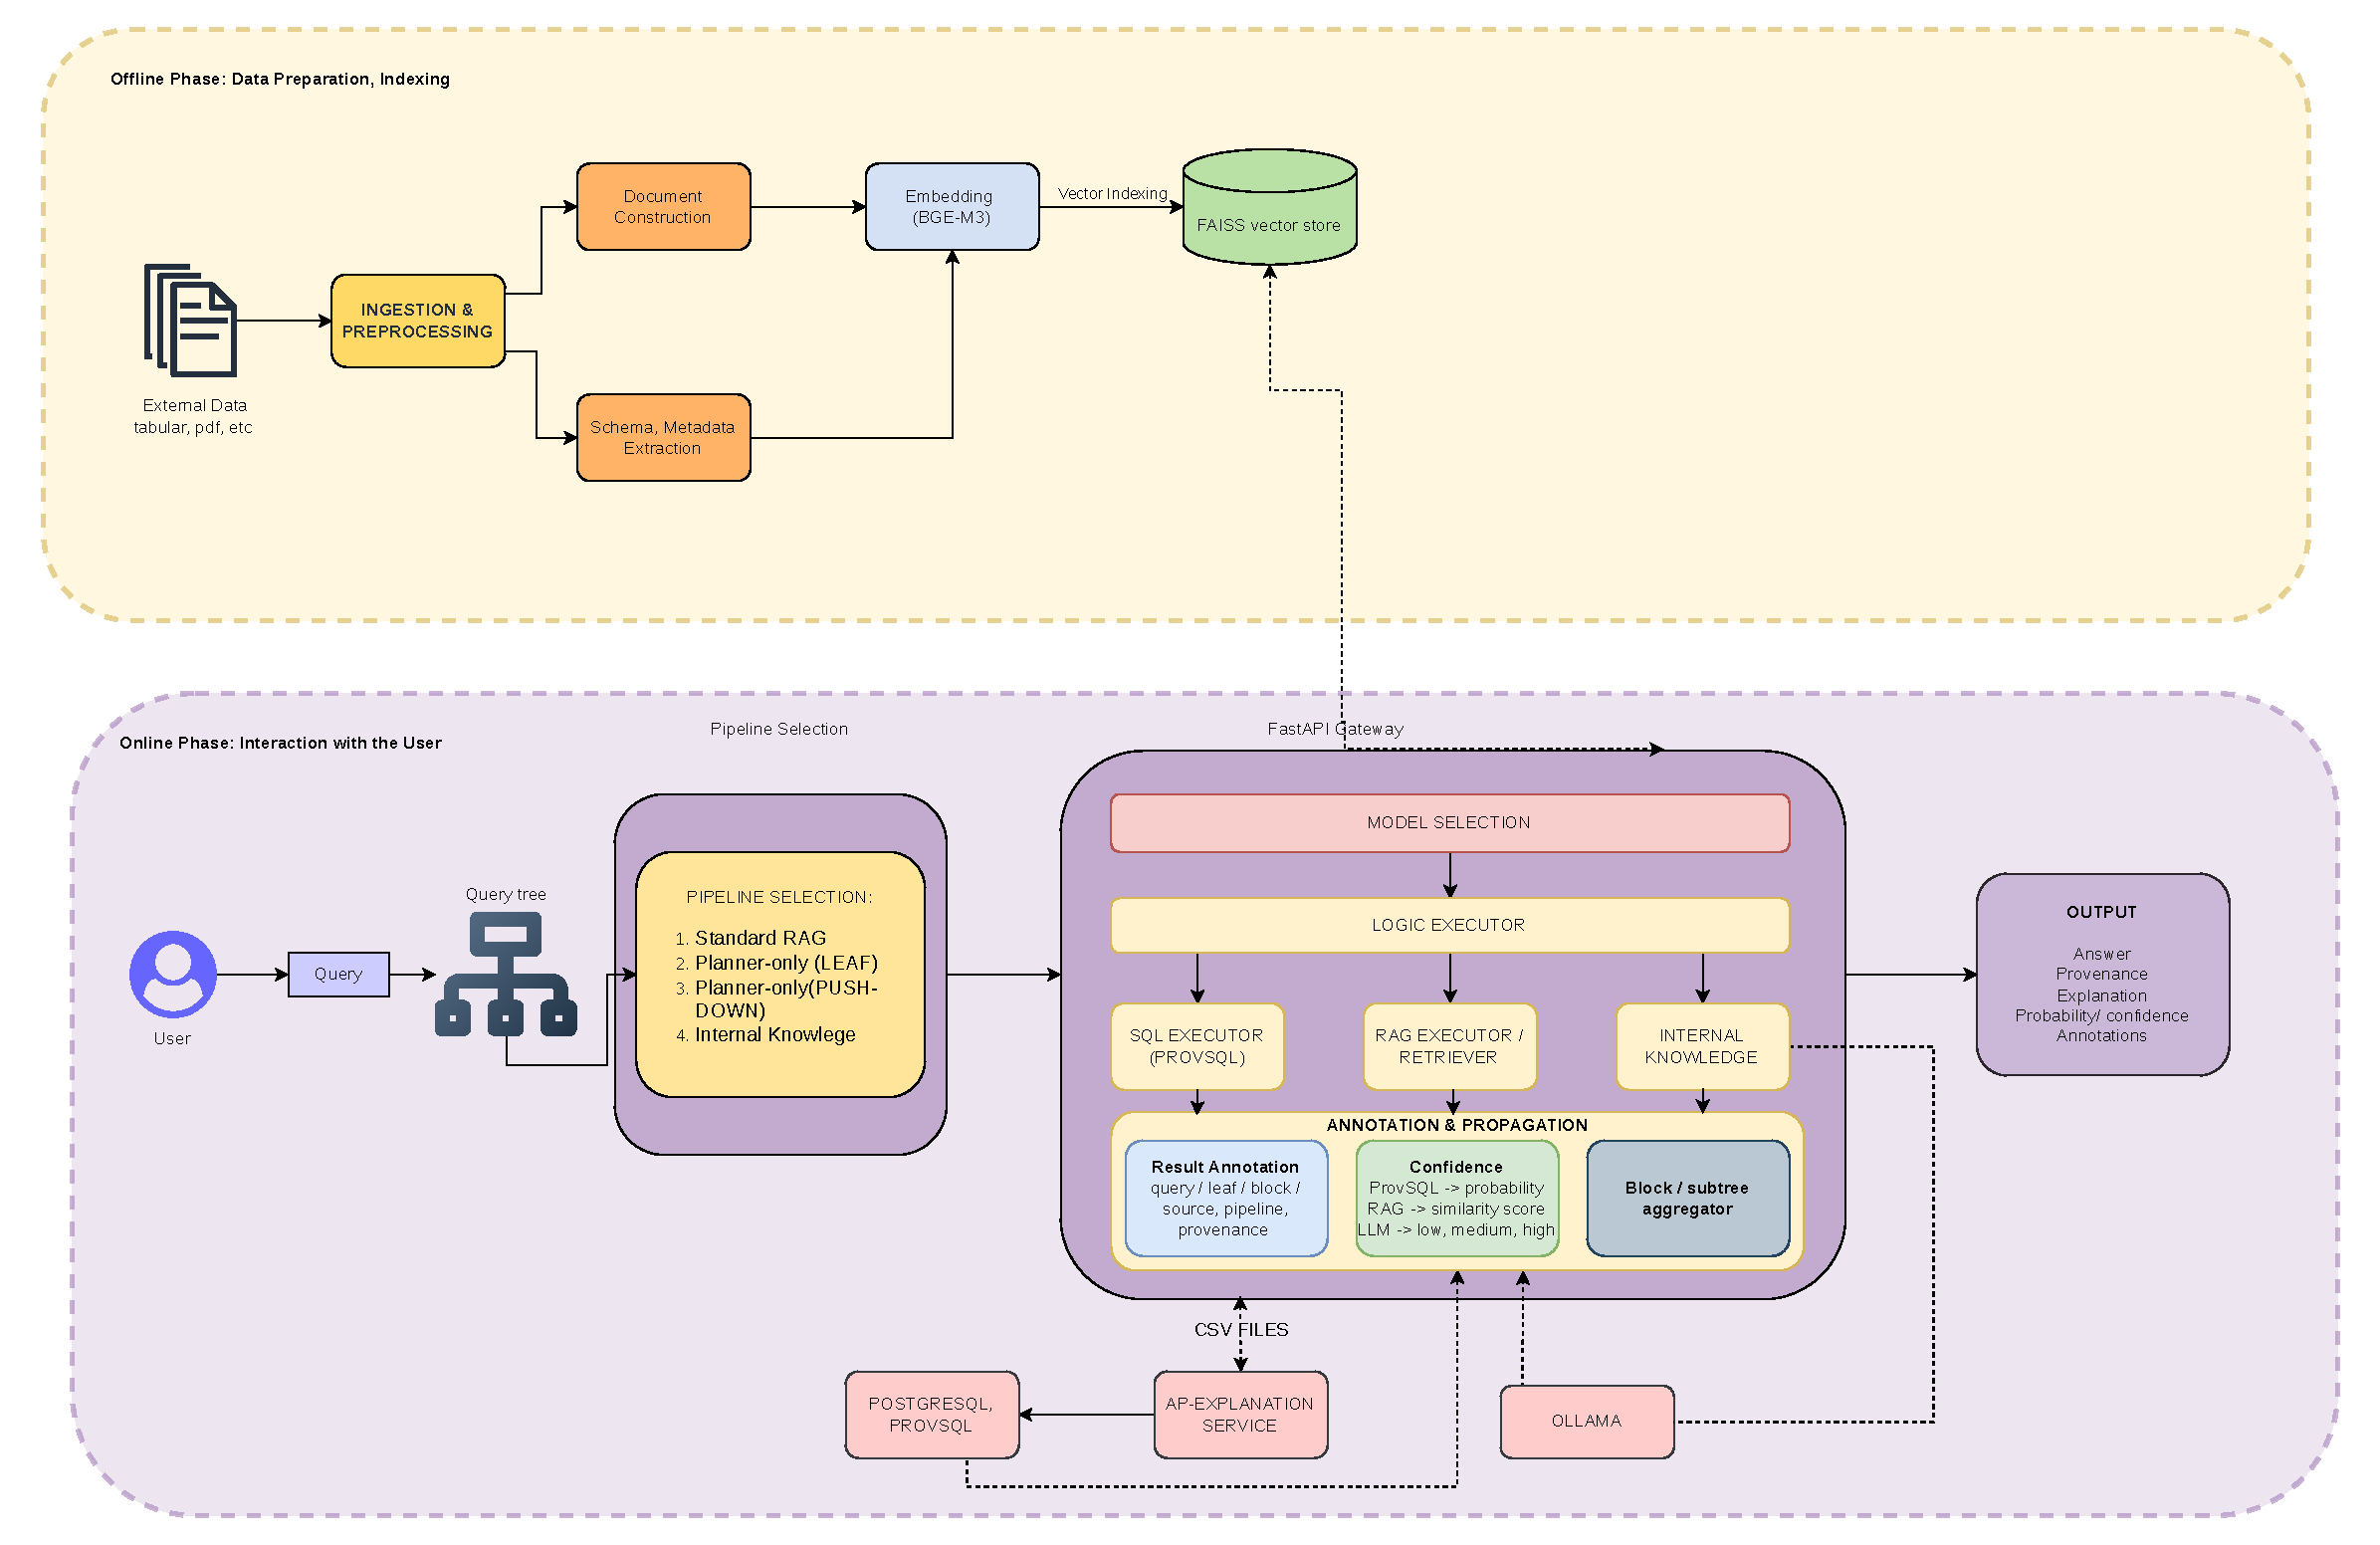
\includegraphics[width=\textwidth]{architecture.pdf}
  \caption{Demo gateway architecture.}
  \label{fig:gateway-architecture}
\end{figure}

\subsection{Main Implementation Files}

\begin{longtable}{>{\raggedright\arraybackslash}p{0.31\textwidth} >{\raggedright\arraybackslash}p{0.61\textwidth}}
\toprule
\textbf{File} & \textbf{Purpose} \\
\midrule
\endhead
\code{gateway.py} & FastAPI application and pipeline orchestration. \\
\code{planner.py} & SQL parsing and structured query-plan construction using \code{sqlglot}. \\
\code{faiss\_index\_manager.py} & Lazy loading, building, checkpointing, and persistence of FAISS indexes. \\
\code{embedding\_strategies.py} & Embedding provider and device selection. \\
\code{prompt.py} & Strict prompts for ordinary and join-aware leaf extraction. \\
\code{iterative\_join\_pipeline.py} & Join-guided ordering, binding propagation, and leaf retrieval. \\
\code{explanation\_pipeline.py} & CSV generation, explanation-service call, and Markdown rendering. \\
\code{explanation\_client.py} & Synchronous and asynchronous AP Explanation API client. \\
\code{json\_to\_csv.py} & Conversion of validated leaf rows into one CSV file per table. \\
\code{prompt\_internal\_knowledge.py} & Dataset-specific prompts for the no-retrieval baseline. \\
\code{ui/} & Browser interface served by the gateway. \\
\bottomrule
\end{longtable}

\section{Data Model and Dataset Handling}

\subsection{Supported Datasets}

The gateway currently defines configurations for:

\begin{itemize}
  \item \code{tpch}, loaded from \code{CSV\_DIR}, with its schema defined in
        \code{tpch\_schema\_info.py}; and
  \item \code{rel-f1}, loaded from \code{RELF1\_CSV\_DIR}, with schema information
        derived from \code{schema\_profile\_relf1.json}.
\end{itemize}

The request field \code{dataset} selects a configuration. If it is omitted,
\code{DEFAULT\_DATASET} is used. Dataset names are normalized before lookup;
unsupported names are rejected.

\subsection{Stable Row Identifiers}

Each CSV table is expected to contain a provenance row-number column such as
\code{nation\_rownum}. During loading, this value is exposed internally as
\code{\_\_rid\_\_} and used as the stable identifier for retrieval, validation,
provenance resolution, and CSV export.

The gateway maintains, separately for each dataset:

\begin{itemize}
  \item an in-memory cache of all loaded rows grouped by table;
  \item a table-local map from row identifier to row position;
  \item a global map from row identifier to the table and row position; and
  \item lazily initialized embedding and FAISS objects.
\end{itemize}

Row identifiers must be globally unambiguous within a dataset for provenance
resolution to be reliable.

\subsection{CSV Loading}

CSV files are loaded lazily. The gateway detects delimiters, reads values as text,
establishes the row identifier, and constructs its lookup indexes. Because CSV
values are textual, the gateway contains dataset-aware SQL rewriting for quoted
identifiers and numeric comparisons before sending some queries to the external
relational service.

\section{Row-Level Indexing and Retrieval}

\subsection{Indexed Representation}

\code{FaissIndexManager} creates one vector document per row. Its text has the form:

\begin{lstlisting}[style=codestyle]
table: nation | n_nationkey: 1 | n_name: ARGENTINA | n_regionkey: 1
\end{lstlisting}

Internal fields such as \code{\_\_rid\_\_} and columns ending in
\code{\_rownum} are excluded from the embedded text. FAISS metadata stores
\code{table} and \code{rid}, allowing the gateway to discard the approximate
document representation and reconstruct the exact row from the CSV cache after
retrieval.

If a non-empty index directory exists, it is loaded. Otherwise, the index is built
in batches and saved for later requests. Consequently, the first request may be
substantially slower.

\subsection{Row Serialization before Embedding}

FAISS does not embed the raw CSV row object directly. Each source row is first
converted into a LangChain \code{Document} containing two separate parts:

\begin{itemize}
  \item \code{page\_content}, the textual representation passed to the embedding
        model; and
  \item \code{metadata}, the structured information retained alongside the vector
        but not included in the embedding unless it is also written explicitly in
        \code{page\_content}.
\end{itemize}

The repository contains two row-serialization workflows. The generic lazy index
builder in \code{FaissIndexManager.row\_to\_text} produces the compact one-line
representation shown above. It prepends the table name, then appends every
non-empty value as \code{column: value}, separated by vertical bars. It excludes
\code{\_\_rid\_\_} and all columns whose names end in \code{\_rownum}. The
associated metadata contains only the table name and row identifier:

\begin{lstlisting}[style=codestyle]
page_content:
table: nation | n_nationkey: 1 | n_name: ARGENTINA | n_regionkey: 1

metadata:
{"table": "nation", "rid": "nation_2"}
\end{lstlisting}

The prebuilt REL-F1 BGE-M3 index uses the richer schema-aware workflow in
\code{build\_row\_index.py}. Its \code{build\_page\_content} function creates a
short natural-language row document with the following sections:

\begin{enumerate}
  \item table identity and a statement that the document represents one row;
  \item primary-key columns and values, when a key candidate is available;
  \item up to 40 non-provenance column values, written with fully qualified names;
  \item outgoing foreign-key relations selected from the schema profile; and
  \item when the referenced row is found, up to four readable values from that row.
\end{enumerate}

For example, a row from the \code{circuits} table is serialized as:

\begin{lstlisting}[style=codestyle]
Row from table circuits.
This row represents one record from circuits.

Primary key:
circuits.circuitId = 1.

Column values:
circuits.circuitId = 1.
circuits.circuitRef = albert_park.
circuits.name = Albert Park Grand Prix Circuit.
circuits.location = Melbourne.
circuits.country = Australia.
circuits.lat = -37.8497.
circuits.lng = 144.968.
circuits.alt = 10.0.
\end{lstlisting}

Provenance columns matching \code{*\_rownum} are not written into this text.
Null values are represented as \code{NULL}; individual textual values are trimmed
and truncated after 120 characters. Foreign-key descriptions have the form
\code{source.column = value references target.column = value}. If the target row
can be resolved, the serializer adds human-readable target attributes, preferring
columns whose names contain terms such as \code{name}, \code{title},
\code{status}, \code{type}, \code{region}, \code{country}, or \code{date}.

The rich document metadata stores \code{doc\_type}, table, generated row ID,
row-number column and value, primary-key values, the complete non-provenance row,
and structured linked-row information. Before building FAISS,
\code{build\_row\_faiss\_index.py} normalizes this metadata by setting
\code{rid} to the provenance row-number value (or, if unavailable, the generated
row ID). This is the identifier expected by the gateway when it resolves a search
result back to the exact CSV row.

The resulting process is therefore:

\begin{center}
CSV row $\longrightarrow$ textual \code{page\_content}
$\longrightarrow$ BGE-M3 dense vector $\longrightarrow$ FAISS,
\end{center}

while the metadata follows the vector into the index and is used only after
retrieval. FAISS similarity search compares the embedded query with the embedded
\code{page\_content}; it does not compare the query directly with the metadata or
the original CSV object.

\subsection{Embedding Models and Strategies}

The embedding backend is selected independently for each dataset. The TPC-H
configuration uses \code{sentence-transformers/all-mpnet-base-v2} by default,
through the Sentence Transformers backend. The REL-F1 row index uses
\textbf{BGE-M3}, configured as \code{BAAI/bge-m3} with the \code{bge-m3}
strategy. BGE-M3 is loaded through \code{FlagEmbedding.BGEM3FlagModel}.

Although BGE-M3 supports multiple retrieval representations, the current gateway
uses only the model's dense vectors (\code{dense\_vecs}) for both document and
query embeddings before FAISS similarity search. Documents are encoded in batches
with a maximum input length of 8192 tokens; queries are encoded individually with
the same maximum length.

The \code{EmbeddingStrategies} wrapper supports three backends:

\begin{itemize}
  \item \code{sentence-transformer}, implemented with \code{SentenceTransformer};
  \item \code{bge-v1.5}, implemented with \code{FlagEmbedding.FlagModel}; and
  \item \code{bge-m3}, implemented with \code{FlagEmbedding.BGEM3FlagModel}.
\end{itemize}

When \code{EMB\_STRATEGY=auto}, the wrapper infers the backend from the model
name: \code{BAAI/bge-m3} selects BGE-M3, other \code{BAAI/bge-*} models select
the BGE v1.5 path, and other names use Sentence Transformers. The shared
\code{EMB\_DEVICE} setting selects CUDA when available or CPU otherwise. BGE
models use half precision on CUDA and full precision on CPU.

The model and strategy used to build an index must also be used when loading and
querying it. Changing either setting requires rebuilding the corresponding FAISS
index; otherwise, vector dimensions or embedding semantics may be incompatible.

\subsection{Retrieval Modes}

The standard RAG path performs one similarity search with \code{RETRIEVER\_K}
candidates and stops after \code{MAX\_CONTEXT\_ROWS} accepted rows. It limits the
context to \code{MAX\_TABLES} distinct tables.

Planner leaf paths use iterative retrieval. The first search requests
\code{RETRIEVER\_K} candidates; each later iteration increases $k$ by the same
amount. Retrieval stops after \code{MAX\_ITERATIVE\_RETRIEVALS} or when an
iteration adds no new resolvable rows. Duplicate identifiers and rows that cannot
be mapped back to the selected dataset are ignored.

When enabled, linked-row metadata may add correlated records up to
\code{MAX\_CORRELATED\_CONTEXT\_ROWS}. Dense retrieval is candidate selection, not
proof of relevance. Exact row validation prevents a model from fabricating row
contents, but it does not guarantee that all rows required for a query were retrieved.

\section{Pipeline Modes}

\subsection{Standard RAG}

The model identifiers \code{base-llama3-8b}, \code{best-ft-llama3-8b-nl}, and
\code{best-ft-llama3-8b-sql} use the standard path:

\begin{enumerate}
  \item The gateway takes the most recent user message as a natural-language question.
  \item It retrieves candidate rows using the complete question.
  \item Exact source rows are serialized into the prompt.
  \item The selected model produces the answer and provenance in a JSON array.
  \item The gateway retries once if the output is not a valid JSON array.
  \item Depending on \code{GATEWAY\_RESPONSE\_FORMAT}, the content is returned as
        raw JSON or rendered Markdown.
\end{enumerate}

This is a useful end-to-end baseline, but answer construction, reasoning, row
selection, and provenance generation remain largely model-controlled.

\subsection{Internal-Knowledge Baseline}

The \code{internal-knowledge} mode does not retrieve source rows. It formats the
question with a dataset-oriented prompt and asks the model to answer from its
internal parameters. Its provenance should not be interpreted as verified source
provenance unless separately resolved and validated.

\subsection{Planner-Only}

The canonical identifier is \code{planner-only}; \code{planner-first} and related
spellings remain compatibility aliases. The input is SQL, not a natural-language
question. \code{build\_query\_plan} parses a \code{SELECT} statement and extracts:

\begin{itemize}
  \item base tables and aliases;
  \item selected columns and local predicates;
  \item join conditions and keys;
  \item grouping columns and aggregates;
  \item ordering and limit;
  \item table-level \code{LeafExtractionTask} objects; and
  \item intended deterministic \code{post\_ops}.
\end{itemize}

For each leaf, the default retrieval query is deliberately broad:

\begin{lstlisting}[style=codestyle]
Retrieve relevant rows for table 'nation'
\end{lstlisting}

The model is instructed to copy rows from the retrieved target-table context. The
gateway returns the plan and complete leaf trace: retrieval query, context, prompt,
raw output, parsed rows, parse error, and validation status.

In the direct \code{planner-only} chat path, the gateway does not execute the
plan's joins, filters, grouping, aggregation, projection, ordering, or limit. A
valid leaf result means that rows were copied faithfully; it does not mean that
the final SQL result was computed.

\subsection{Planner-Only with Predicate Pushdown}

\code{planner-only-pushdown} uses the same planner and leaf contract, but includes
local predicate text and required columns in each retrieval query. This exposes
entity names and filter values to FAISS and can improve candidate recall for
selective predicates.

This mode is selectable per leaf through the UI workflow. The chat endpoint does
not have a separate top-level planner branch for this identifier; a direct chat
request falls through to standard RAG behavior. Clients requiring planner
pushdown should therefore use the UI run API unless that routing is changed.

\subsection{Iterative Join-Aware Pipeline}

\code{iterative-join-aware} uses the SQL plan to coordinate retrieval across joined tables:

\begin{enumerate}
  \item select a starting leaf, preferring tasks with useful local predicates or join keys;
  \item extract validated rows for that table;
  \item propagate join-key values as bindings to connected tables;
  \item enrich the next retrieval query with inherited values and source-row information;
  \item repeat until every planned table has been processed; and
  \item write the extracted relations to CSV and call the AP Explanation service.
\end{enumerate}

Each leaf output records its step number, inherited bindings, and source row
identifiers. The algorithm improves join-aware candidate discovery but remains
dependent on the first leaf's recall and on correctly extracted join edges.

\subsection{Planner-Only Explanation}

\code{planner-only-explanation} extends planner-only extraction with an external
deterministic stage:

\begin{enumerate}
  \item run the planner-only leaf pipeline;
  \item retain validated, parsed rows;
  \item remove \code{\_\_rid\_\_} and write one CSV per table;
  \item submit the SQL query and CSV file list to the AP Explanation service;
  \item poll asynchronous jobs until success, failure, or timeout; and
  \item return the service output as Markdown.
\end{enumerate}

The row-number column is retained by default so provenance can be mapped back to
the original rows. Empty or invalid leaf outputs may cause missing CSV relations
and an incomplete or failed downstream query.

\section{Leaf Output Contract and Validation}

A leaf model must return a JSON array containing objects with exactly two keys:

\begin{lstlisting}[style=codestyle]
[
  {
    "row_id": "nation_2",
    "values": {
      "nation_rownum": "nation_2",
      "n_nationkey": "1",
      "n_name": "ARGENTINA",
      "n_regionkey": "1",
      "__rid__": "nation_2"
    }
  }
]
\end{lstlisting}

Validation checks that:

\begin{itemize}
  \item the root is an array;
  \item every item is an object with exactly \code{row\_id} and \code{values};
  \item \code{row\_id} is a string present in the retrieved target-table context;
  \item valid row identifiers are not duplicated;
  \item \code{values} exactly equals the corresponding source row; and
  \item \code{values.\_\_rid\_\_}, when present, equals \code{row\_id}.
\end{itemize}

The model is called at most twice. On failure, the second prompt emphasizes the
JSON-only contract. The partial parser retains individually valid rows even if the
complete output is invalid, enabling evaluation and downstream inspection without
silently treating malformed items as trusted data.

\section{API}

\subsection{OpenAI-Compatible Endpoints}

\subsubsection{\code{GET /v1/models}}

This endpoint returns logical identifiers rather than provider-specific model tags:

\begin{lstlisting}[style=codestyle]
base-llama3-8b
best-ft-llama3-8b-nl
best-ft-llama3-8b-sql
planner-only
planner-only-pushdown
planner-only-explanation
internal-knowledge
iterative-join-aware
\end{lstlisting}

\subsubsection{\code{POST /v1/chat/completions}}

Accepted fields include \code{model}, \code{messages}, \code{temperature},
\code{stream}, and \code{dataset}. Extra fields are accepted for client
compatibility. The gateway uses only the latest message whose role is \code{user}.

\begin{lstlisting}[style=codestyle]
curl -X POST http://localhost:9006/v1/chat/completions \
  -H 'Content-Type: application/json' \
  -d '{
    "model": "planner-only",
    "dataset": "tpch",
    "messages": [{"role": "user", "content": "SELECT n_name FROM nation"}],
    "temperature": 0
  }'
\end{lstlisting}

The response follows the non-streaming OpenAI chat-completion envelope. Token
counts are placeholders and return zero. Although the schema accepts
\code{stream}, this endpoint does not emit OpenAI streaming chunks.

\subsection{Provenance Explanation Endpoint}

\code{POST /v1/provenance/explain} accepts a natural-language question and a
previously generated answer JSON string. It parses the result/provenance array,
resolves identifiers, detects structural problems, renders provenance expressions,
and requests a concise domain explanation when all identifiers resolve. If any
identifier is missing, model-based explanation is skipped and validation errors
are returned.

\subsection{Browser UI Endpoints}

\begin{longtable}{>{\raggedright\arraybackslash}p{0.32\textwidth} >{\raggedright\arraybackslash}p{0.60\textwidth}}
\toprule
\textbf{Endpoint} & \textbf{Purpose} \\
\midrule
\endhead
\code{GET /} & Redirect to \code{/ui}. \\
\code{GET /ui} & Serve the interactive workspace. \\
\code{POST /ui/plan} & Build and return a SQL plan. \\
\code{POST /ui/run} & Run selected per-leaf pipelines and AP explanation synchronously. \\
\code{POST /ui/run/stream} & Emit NDJSON progress events and a final result. \\
\code{GET /ui/csv} & Inspect generated CSV files in the shared bucket. \\
\code{GET /debug/ui} & Inspect the latest in-memory chat and provenance-debug state. \\
\bottomrule
\end{longtable}

The streaming UI endpoint uses NDJSON (\code{application/x-ndjson}), not
Server-Sent Events and not the OpenAI streaming protocol.

\section{Model Routing and Providers}

Logical identifiers keep clients stable while environment variables select
concrete models. Base and fine-tuned modes normally route to Ollama. Planner leaf
calls use \code{PLANNER\_LLM\_PROVIDER}, which may be \code{ollama},
\code{openai}, or \code{openai-compatible}. A compatible remote provider uses
\code{LLM\_API\_BASE}, \code{LLM\_API\_KEY}, \code{LLM\_API\_MODEL}, request
timeout, and TLS verification settings.

Temperature defaults to $0.0$. Authentication headers received by the gateway are
not used to protect these endpoints; deployment-level access control is required
outside a trusted local environment.

\section{Configuration Reference}

\begin{longtable}{>{\raggedright\arraybackslash}p{0.20\textwidth} >{\raggedright\arraybackslash}p{0.72\textwidth}}
\toprule
\textbf{Area} & \textbf{Variables} \\
\midrule
\endhead
Dataset & \code{DEFAULT\_DATASET}, \code{CSV\_DIR}, \code{RELF1\_CSV\_DIR}, \code{RELF1\_SCHEMA\_PROFILE}. \\
FAISS & \code{FAISS\_INDEX\_FOLDER}, \code{RELF1\_FAISS\_INDEX\_FOLDER}, \code{INDEX\_TABLES}, \code{RELF1\_INDEX\_TABLES}, \code{INDEX\_BATCH\_SIZE}. \\
Embeddings & \code{EMB\_MODEL}, \code{EMB\_STRATEGY}, \code{EMB\_DEVICE}, \code{RELF1\_EMB\_MODEL}, \code{RELF1\_EMB\_STRATEGY}. \\
Retrieval & \code{RETRIEVER\_K}, \code{MAX\_ITERATIVE\_RETRIEVALS}, \code{MAX\_CONTEXT\_ROWS}, \code{MAX\_TABLES}, \code{INCLUDE\_CORRELATED\_CONTEXT\_ROWS}, \code{MAX\_CORRELATED\_CONTEXT\_ROWS}. \\
Ollama & \code{OLLAMA\_HOST}, \code{OLLAMA\_NUM\_CTX}, \code{OLLAMA\_REQUEST\_TIMEOUT}, and model-specific \code{OLLAMA\_MODEL\_*} variables. \\
Compatible LLM & \code{PLANNER\_LLM\_PROVIDER}, \code{PLANNER\_LLM\_MODEL}, \code{LLM\_API\_BASE}, \code{LLM\_API\_KEY}, \code{LLM\_API\_MODEL}, \code{LLM\_SSL\_VERIFY}, \code{LLM\_REQUEST\_TIMEOUT}. \\
Explanation & \code{EXPLANATION\_URL}, \code{EXPLANATION\_ENDPOINT}, \code{EXPLANATION\_BUCKET\_DIR}, \code{EXPLANATION\_REQUEST\_TIMEOUT}, \code{EXPLANATION\_CSV\_DELIMITER}, \code{EXPLANATION\_KEEP\_ROWNUM}. \\
Rendering and logging & \code{GATEWAY\_RESPONSE\_FORMAT}, \code{GATEWAY\_MARKDOWN\_INCLUDE\_RAW}, \code{GATEWAY\_MARKDOWN\_MAX\_ROWS}, \code{GATEWAY\_LOG\_PATH}. \\
\bottomrule
\end{longtable}

\section{Deployment and Operation}

\subsection{Prerequisites}

\begin{itemize}
  \item Docker with Compose support;
  \item Git and Git LFS for the fine-tuned model artifacts;
  \item sufficient disk and memory for model serving and embedding indexes; and
  \item network access to any configured remote LLM endpoint.
\end{itemize}

\subsection{Starting the Stack}

\begin{lstlisting}[style=codestyle]
git lfs pull
docker compose up -d --build
docker compose ps
\end{lstlisting}

The current Compose mapping exposes the gateway on \code{127.0.0.1:9006}, the
explanation service on host port \code{5002}, and keeps Ollama internal to the
Compose network. The \code{ollama-init} service waits for Ollama, pulls the base
model if needed, and creates fine-tuned model tags from their \code{Modelfile}
definitions.

\begin{lstlisting}[style=codestyle]
docker compose logs -f gateway
\end{lstlisting}

\subsection{Persistence}

\begin{itemize}
  \item Ollama model data is stored in the \code{ollama\_data} volume.
  \item PostgreSQL state is stored in \code{wp4\_poc\_postgres\_data}.
  \item Indexes, datasets, logs, UI files, and the shared CSV bucket are
        bind-mounted from the repository.
\end{itemize}

\section{Observability and Error Behavior}

The gateway writes JSON Lines events to \code{GATEWAY\_LOG\_PATH}. Events include
request metadata, selected dataset and model, retrieval iterations, row
identifiers, contexts, planner results, prompts, raw model outputs, validation
status, generated files, explanation output, and errors.

\code{/debug/ui} stores only the latest debug state in process memory. It is
overwritten by later requests, is not durable, and may expose source data and
prompts. Logs and debug endpoints should be treated as sensitive outside a demo.

Explicitly handled client errors return HTTP 400. Pipeline and provider failures
generally return HTTP 500. The UI streaming endpoint instead emits structured
\code{error} or \code{fatal\_error} events so the browser can show partial progress.

\
\bibliographystyle{plain}
\bibliography{bibfile}

\end{document}
